%##########################################################################
%##########################  CHAPER 6: APPLICATION  #######################
%##########################################################################

\chapter{Entwicklung der Anwendung}\label{kap:application}

In diesem Kapitel wird die Entwicklung der Applikation als Autonomes 
und on the Edge System auf dem Respberry Pi zusammen mit dem ncs2 und einer 
geeigneten Kamera beschrieben.
Ebenso die Integration des trainierten Tensorflow Models in Appl sowie 
eine Möglichkeit mit dem System über eine Netzwerk Verbindung zu kommunizieren.


%##########################  SECTION 1: AUFBAU  ###########################
\section{Aufbau}\label{sec:aufbau}

Die Anwendung soll auf einem Raspberry Pi 4 Abbildung \ref{subfig:raspy} 
laufen, an den die nötigen Komponenten angeschlossen werden. Dazu 
ghören der Neural Compute Stick 2, zur Ausführung der Inferenz, ein 
Kamera Modul, mit welchem die Bilder aufgenommen werden, sowie ein 
WiFi Stick und Powrebank.
\\
Der Neural Compute Stick wird über USB angeschlossen und kann 
nach installation des OpenVino Toolkits verwendet werden.
\\
Als Kamera wird RPiCam Modul verwendet, welches über ein \dots 
Kabel an den \dots Eingang des Raspberrys verbunden wird.


\begin{figure}[htb]
    \centering
    \begin{subfigure}{6cm}
        \centering
        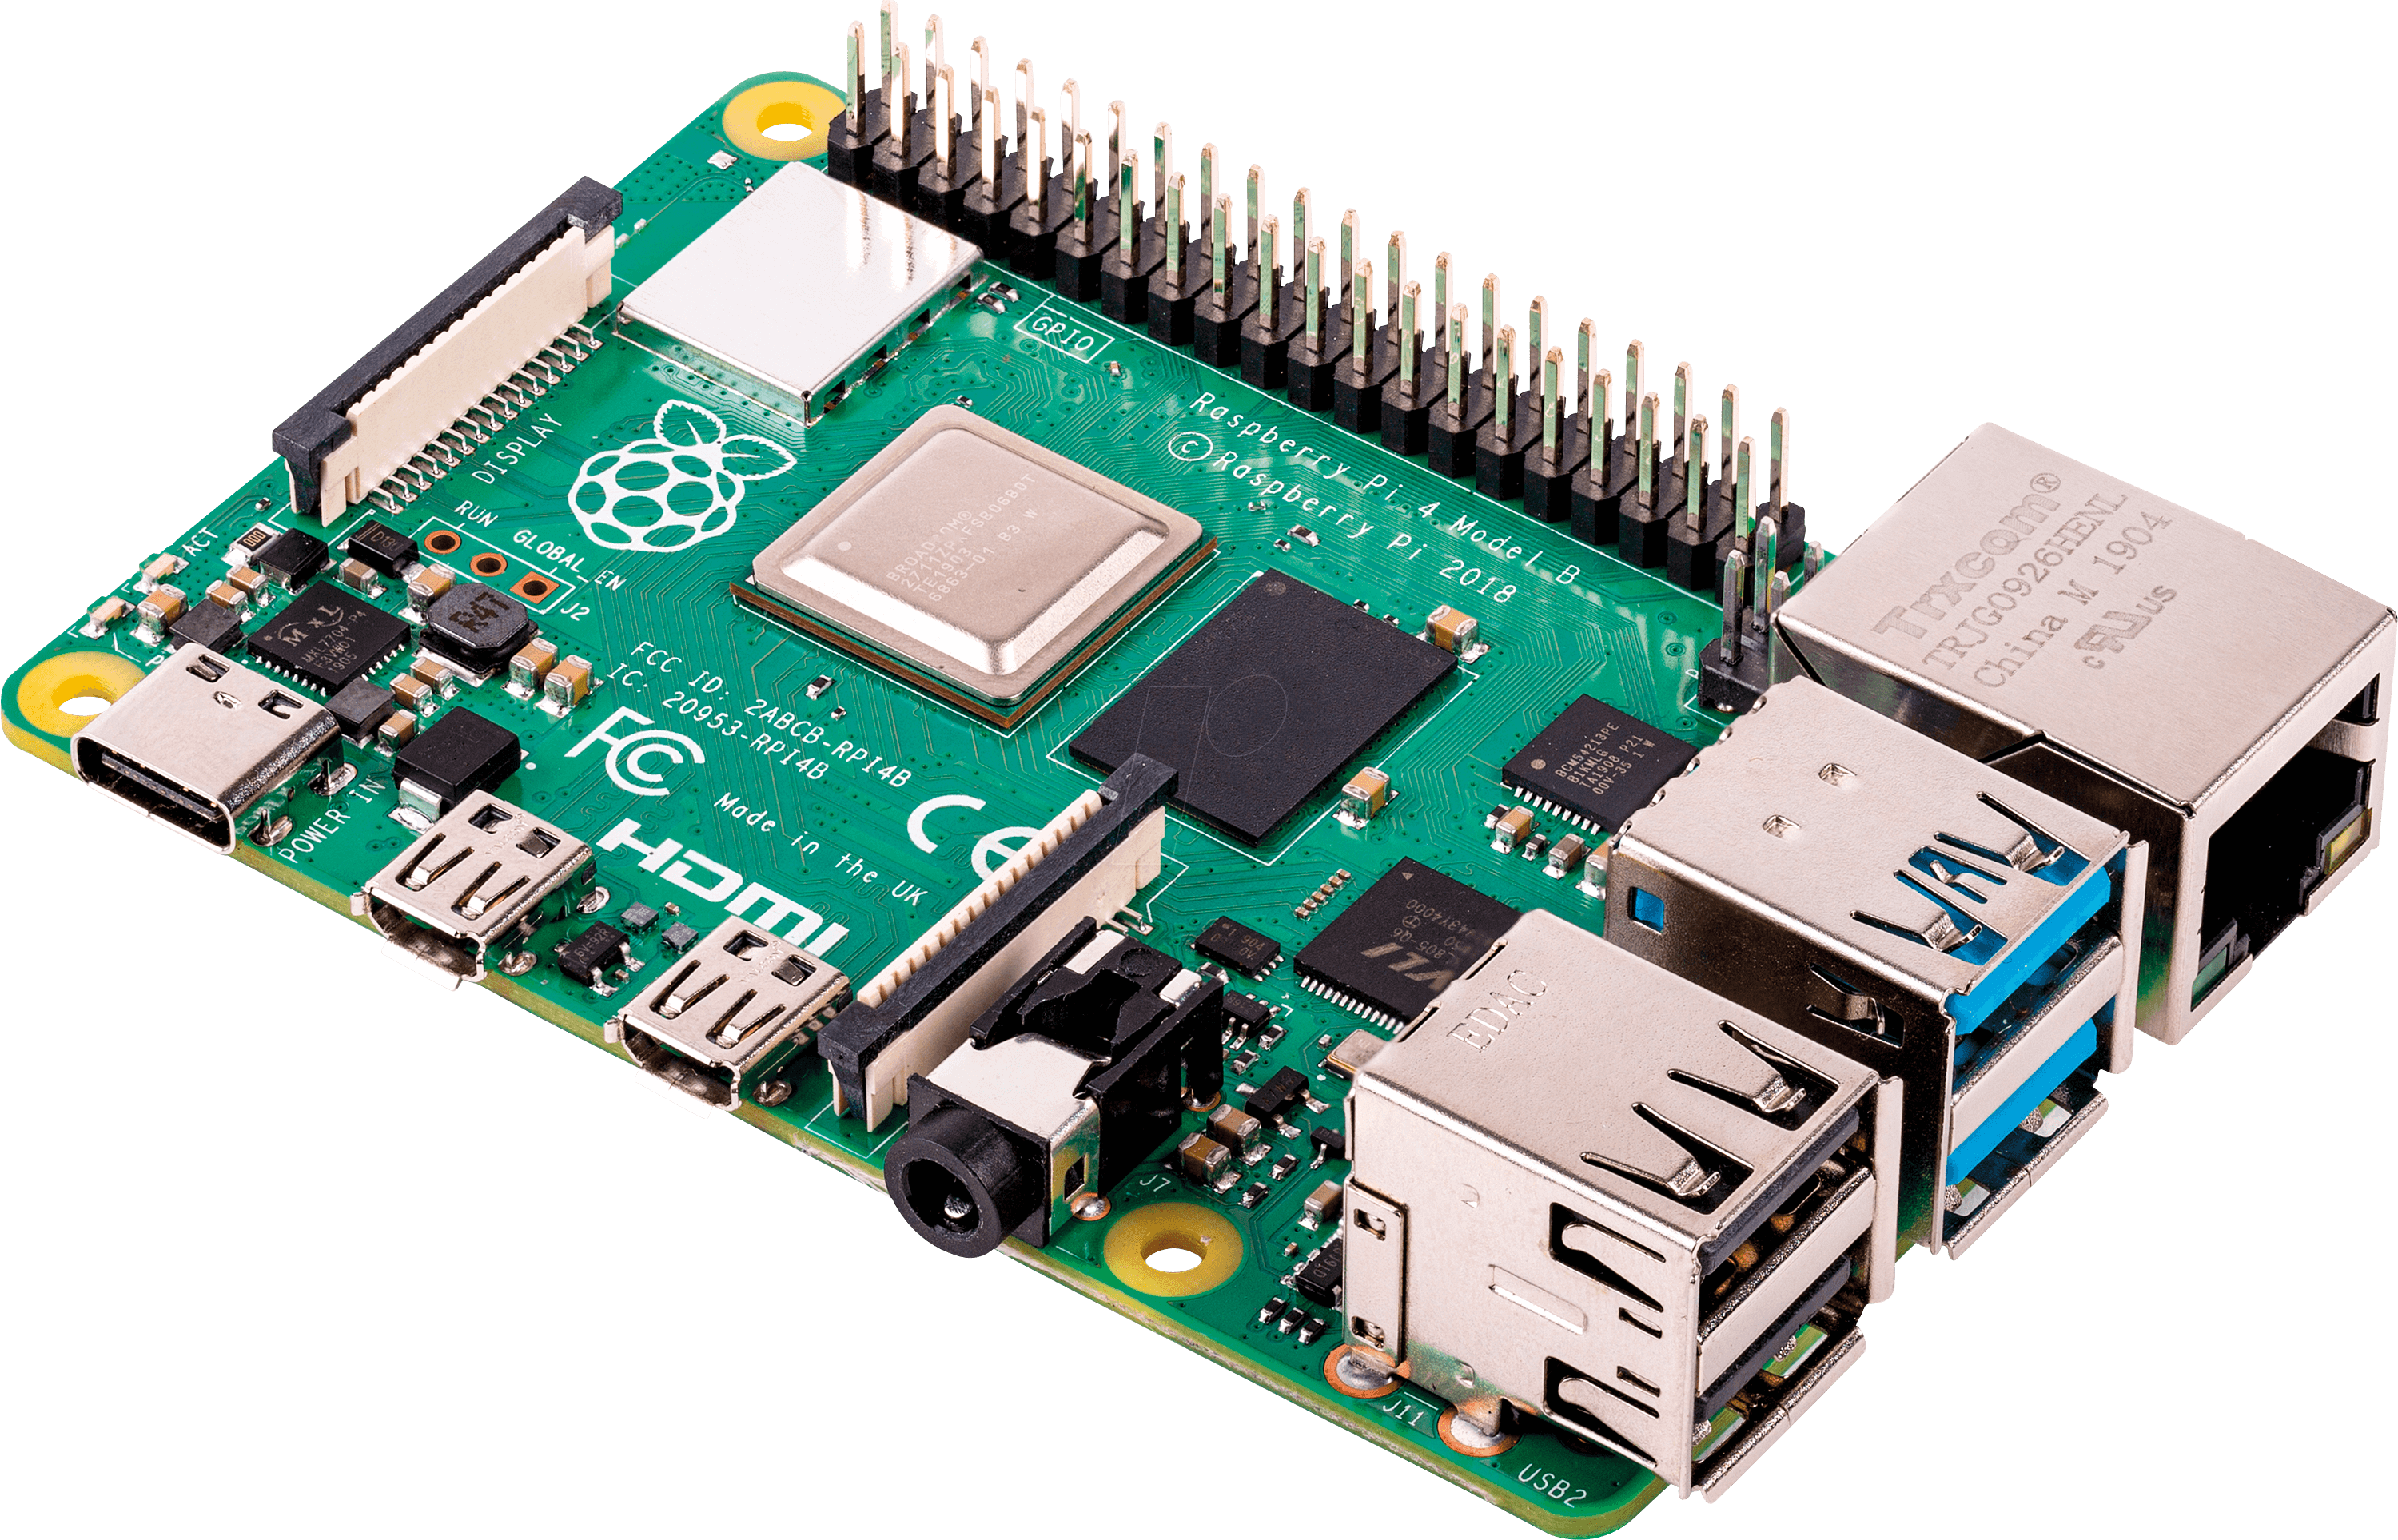
\includegraphics[width=5cm]{./Bilder/raspberrypi_4.png}
        \subcaption{RaspberryPi 4}
        \label{subfig:raspy}
    \end{subfigure}
    \begin{subfigure}{6cm}
        \centering
        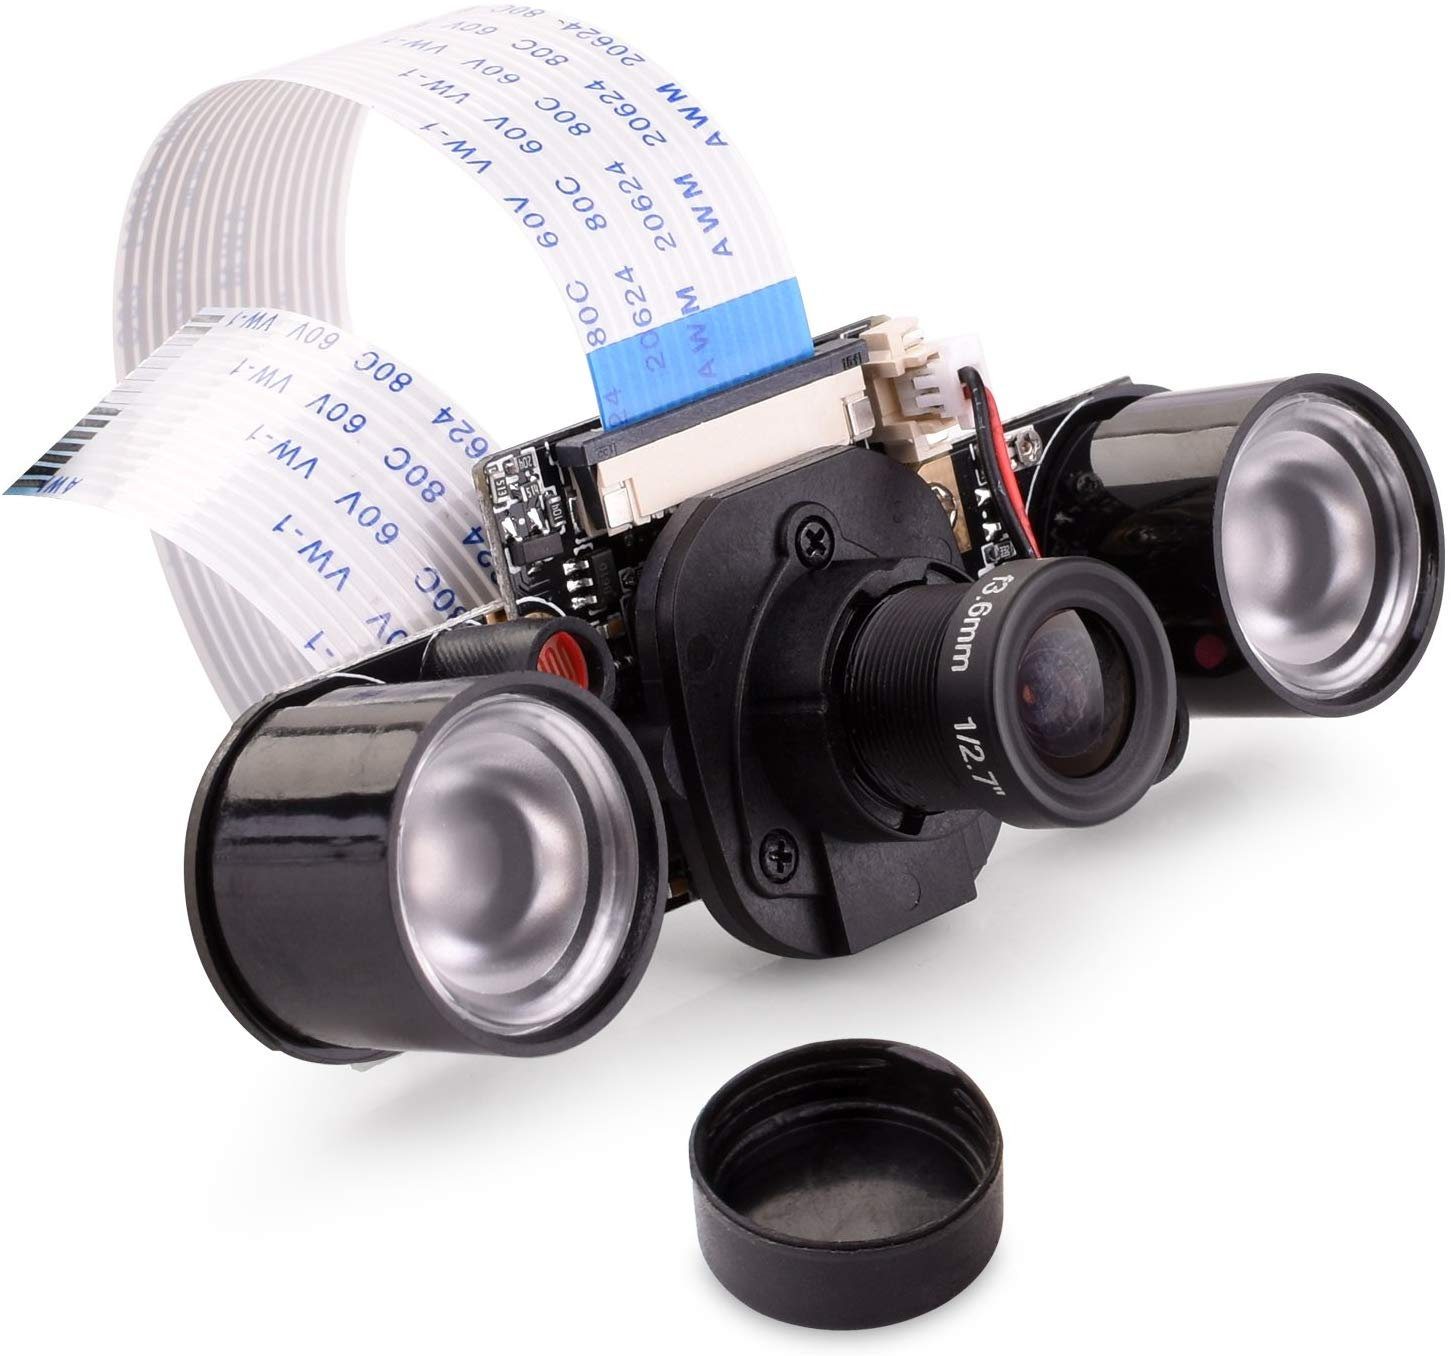
\includegraphics[width=4cm]{./Bilder/RPiCam.jpg}
        \subcaption{Quimat Raspberry Pi Kamera}
        \label{subfig:rpicam}
    \end{subfigure}
    \label{img:raspy_cam}
\end{figure}


Für die Spannungsversorgung \dots berechnung aus verbrauch von ncs2 + 
kamera + ir leds mal zeit. Ergibt folgende Laufzeit.\\
Für die Netzwerk Verbindung \dots um die Erkannten Bilder via 
Client-Server-Verbindung an einen Host Pc übermitteln zu können.\\

Die folgenden Abschnitte beschreiben die Implementierung um die in Kapitel 
\ref{kap:anforderunganalyse} beschriebenen Anforderungen zu realisieren.
\\
Die über das Kamera Modul aufgenommen Bilder mit dem in Kapitel 
\ref{kap:objerk} trainierten Neuronalen Netz zu inferieren und Bilder 
der erkannte Objekte an zweiten Computer zu senden.

%----------------------------------------------------------------------




%##########################  SECTION 2: OPENVINO  #######################
\section{OpenVino Toolkit}\label{sec:openvino}

Die Implementierung der Inferenz des trainierten Models wurde 
mithilfe des OpenVino Toolkits vorgenommen, eine \dots von Intel, 
welche die Inferenz auf verschiedener Hardware Unterstützt, darunter 
auch die MYRIAD Vpu des Neural Compute Sticks 2. Das Toolkit 
verwendet dabei ein eigenes, vom Framework unabhängigen Dateiformat 
für die Modelle, die sog Intermediate Representation.

Das Toolkit besteht im Wesentlichen aus den zwei Komponenten 
\textit{Model Optimizer} und \textit{Inference Engine}



Die implementierung der auf dem RaspberryPi auszuführenden 
Application/Software wurde in Python vorgenommen.

Mit dem Model Optimizer können Modelle der Frameworks Tensorflow, 
Caffee, \dots in das IR Format konvertiert werden. Diese besteht 
aus einer .xml Datei, welche die Struktur/Architektur des Modell 
enthällt sowie einer .bin Datei, mit den trainierten Gewichten.

\begin{figure}[htb]
    \centering
    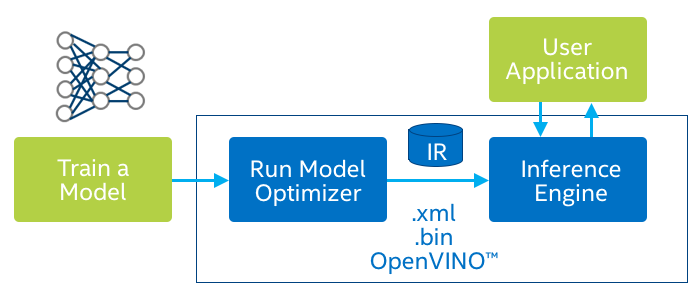
\includegraphics[width=10cm]{./Bilder/open_vino_workflow_steps.png}
    \caption{Workflow: OpenVino Toolkit}
    \label{img:ov_workflow}
\end{figure}

Die InferenceEngine, welche in der User Application implementiert 
wird, lädt die IR Dateien in ein Plugin, über das nun die Inferenz 
auf Input Daten ausgeführt werden kann.

%----------------------------------------------------------------------


%##########################  SECTION 3: KAMERA  ########################
\section{Raspberry Pi Kamera}\label{sec:raspicam}


Bei der Kamera handelt es sich um das OV5647 5MP Modul mit regelbarem 
Infrarotfilter. Zusammen mit zwei Infrarot LEDs von der Firma Quimat 
Abbildung \ref{subfig:rpicam}
\\
Wird der Infrarotfilter ausgeschaltet ist es durch die Infrarot LEDs mit 
850nm welligen Licht möglich auch bei dunkelheit aufnahmen zu machen, 
die in Graustufen Werten dargestellt werden.

%------------------------------------------------------------------------


%##########################  SECTION 4: CONNECTION  #####################
\section{Server-Client-Connection}\label{sec:serverclient}



%------------------------------------------------------------------------


%##########################  SECTION 1: REST  ###########################
\section{put it all together}\label{sec:ka}



%-------------------------------------------------------------------------




